% ============================================================================
%  অধ্যায় ৪ — ফাংশন ১
%  COMPILE WITH XeLaTeX  (twice, so the point total resolves)
%  Overleaf: Menu -> Compiler -> XeLaTeX
%  Requires: bnhandout.sty  and  fonts/Kalpurush.ttf  in the project
% ============================================================================
\documentclass[11pt]{article}
\usepackage{bnhandout}

\usepackage{amsmath}
\usepackage{amssymb}
\usepackage{tikz}

\hauthor[https://sites.google.com/view/jugantordey]{Jugantor Dey}
\hseries{\textit{Mathematics for the Physics Olympiad}}

\begin{document}

\handouttitle{Chapter 4 : Function I}

\noindent
এই অধ্যায়ে শুরুর আগে অধ্যায় ২ (Algebra I) শেষ করে নাও। চলক,
রাশি, অভেদ বনাম সমীকরণ, আর সরল সমীকরণ সমাধান করতে পারা এখানে ধরে নেওয়া
হয়েছে। কয়েকটি উদাহরণ ও সমস্যায় মধ্যপদ বিশ্লেষণ আর বর্গমূল লেগেছে, যা
অধ্যায় ৩-এর বিষয়; ওগুলো এখনো না পড়ে থাকলে সেই কটা জায়গা আপাতত এড়িয়ে
গেলেও বাকিটুকু বুঝতে অসুবিধা হবে না।

\noindent এই সিরিজের মেরুদণ্ডই হলো function। limit, derivative, integral, vector,
vector calculus; সবকিছুই আসলে function নিয়ে করা কাজ। তাই এখানে
সংজ্ঞাগুলো একটু ধীরে, একটু বেশি যত্ন নিয়ে গড়া হয়েছে। মুখস্থ করার কিছু নেই;
প্রতিটি সংজ্ঞা কেন ঠিক ওভাবেই লেখা হয়েছে, সেটা ধরতে পারলেই কাজ শেষ।

\noindent একটা কথা আগেই বলে রাখি। function-এর লেখচিত্র (graph) এখানে ইচ্ছে করেই
ব্যবহার করা হয়নি, কারণ কার্তেসীয় সমতল গড়ে তোলা হবে অধ্যায় ৬-এ। তার
বদলে এখানে তীরচিহ্নের ছবি (arrow diagram) দিয়ে কাজ চালানো হয়েছে
এবং সত্যি বলতে, এই অধ্যায়ের মূল ধারণাগুলোর জন্য ওই ছবিই লেখচিত্রের
চেয়ে ভালো।

\noindent এই অধ্যায়ে মোট \totalpoints\ পয়েন্ট আছে।

% ============================================================================
\section{সেট ও ব্যবধি}
% ============================================================================

Function-এর সংজ্ঞা লিখতে গেলে প্রথমেই বলতে হয় `কী কী ইনপুট দেওয়া যাবে''
আর ``কী কী আউটপুট আসতে পারে''। অর্থাৎ দুটো সংগ্রহের কথা বলতে হয়। তাই
শুরুটা set দিয়ে।

\begin{idea}[সেট]
Set হলো কতগুলো বস্তুর একটা সংগ্রহ। বস্তুগুলোকে বলে সেটটির উপাদান (element)।
$S$ একটি set হলে $a \in S$ লিখে বোঝায় $a$ হলো $S$-এর একটি উপাদান, আর
$a \notin S$ লিখে বোঝায় $a$ হলো $S$-এর উপাদান নয়।

Set লেখার দুটো চেনা উপায় আছে। উপাদানগুলো একে একে লিখে দেওয়া যায়:
\[
  A = \{1, 2, 3, 4, 5, 6\},
\]
অথবা শর্ত দিয়ে বলা যায় কারা কারা এর ভেতরে পড়ে:
\[
  A = \{\, x : x \text{ পূর্ণসংখ্যা এবং } 0 < x < 7 \,\}.
\]
দ্বিতীয়টিকে বলে set-builder notation, আর পড়া হয় ``$A$ হলো সেই সব $x$-এর set,
যারা পূর্ণসংখ্যা এবং $0$ ও $7$-এর মাঝে''। :-কে পড়া হয় "such that"। আর প্রথমটিকে বলে list notation।

যে set-এ একটিও উপাদান নেই তাকে বলে ফাঁকা set, লেখা হয় $\emptyset$ বা $\{\}$।
$S$-এর প্রতিটি উপাদান যদি $T$-এরও উপাদান হয়, তবে $S$ হলো $T$-এর উপসেট, লেখা
হয় $S \subseteq T$।

দুটি set $S$ ও $T$ থেকে নতুন set বানানো যায়:
\[
  S \cup T = \{\, x : x \in S \text{ অথবা } x \in T \,\}, \qquad
  S \cap T = \{\, x : x \in S \text{ এবং } x \in T \,\}.
\]
প্রথমটি সংযোগ (union), দ্বিতীয়টি ছেদ (intersection)।
\end{idea}

\noindent
কিছু set এত ঘন ঘন লাগে যে তাদের নিজস্ব চিহ্ন আছে, আর এই সিরিজে সেগুলোই
ব্যবহার করা হবে:
\[
  \mathbb{N} = \{1, 2, 3, \dots\}, \qquad
  \mathbb{Z} = \{\dots, -2, -1, 0, 1, 2, \dots\}, \qquad
  \mathbb{Q} = \Big\{ \tfrac{p}{q} : p, q \in \mathbb{Z},\ q \neq 0 \Big\} \text{(মূলদ সংখ্যার সেট)},
\]
আর $\mathbb{R}$ দিয়ে বোঝানো হয় সব বাস্তব সংখ্যার set। স্পষ্টতই
$\mathbb{N} \subseteq \mathbb{Z} \subseteq \mathbb{Q} \subseteq \mathbb{R}$।

\begin{idea}[ব্যবধি]
বাস্তব সংখ্যার কিছু set এত বেশি লাগে যে তাদের জন্য আলাদা সংক্ষিপ্ত লেখা আছে।
$a < b$ হলে
\[
  (a, b) = \{\, x \in \mathbb{R} : a < x < b \,\}, \qquad
  [a, b] = \{\, x \in \mathbb{R} : a \leq x \leq b \,\}.
\]
প্রথমটিকে বলে খোলা ব্যবধি (open interval), দ্বিতীয়টিকে বদ্ধ ব্যবধি (closed
interval)। প্রথম বন্ধনী মানে প্রান্তবিন্দুটি বাদ, তৃতীয় বন্ধনী মানে
প্রান্তবিন্দুটি সহ। এক পাশ খোলা আর এক পাশ বদ্ধও হতে পারে:
$[a, b)$ এবং $(a, b]$।

অসীম পর্যন্ত বিস্তৃত ব্যবধিও লেখা যায়:
\[
  (a, \infty) = \{\, x : x > a \,\}, \qquad
  (-\infty, b] = \{\, x : x \leq b \,\}, \qquad
  (-\infty, \infty) = \mathbb{R}.
\]
\end{idea}

\begin{center}
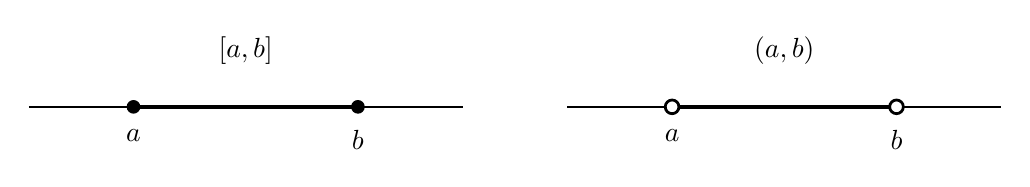
\begin{tikzpicture}[scale=0.95]
  % closed interval
  \draw[thick] (-0.4,0) -- (5.4,0);
  \draw[line width=1.6pt] (1,0) -- (4,0);
  \fill (1,0) circle (2.6pt);
  \fill (4,0) circle (2.6pt);
  \node[below] at (1,-0.18) {$a$};
  \node[below] at (4,-0.18) {$b$};
  \node at (2.5,0.75) {$[a,b]$};
  % open interval
  \begin{scope}[xshift=7.2cm]
    \draw[thick] (-0.4,0) -- (5.4,0);
    \draw[line width=1.6pt] (1,0) -- (4,0);
    \draw[fill=white,line width=1pt] (1,0) circle (2.6pt);
    \draw[fill=white,line width=1pt] (4,0) circle (2.6pt);
    \node[below] at (1,-0.18) {$a$};
    \node[below] at (4,-0.18) {$b$};
    \node at (2.5,0.75) {$(a,b)$};
  \end{scope}
\end{tikzpicture}
\end{center}

\noindent
ভরাট বিন্দু মানে প্রান্তবিন্দুটি set-এর ভেতরে, ফাঁকা বিন্দু মানে বাইরে।

\begin{remark}
$\infty$ কোনো সংখ্যা নয়। $(a, \infty)$ লেখাটা একটামাত্র জিনিস বোঝায় :
``$a$-এর চেয়ে বড় সব বাস্তব সংখ্যা''। তাই $[a, \infty]$ লেখা অর্থহীন, কারণ
তৃতীয় বন্ধনী বলছে প্রান্তবিন্দুটি set-এর ভেতরে আছে, অথচ $\infty$ নামে কোনো
সংখ্যাই তো নেই যে সে ভেতরে থাকবে। তাই অসীমের দিকে সবসময় প্রথম বন্ধনী।

পরে অধ্যায় ১৪-এ যখন $x \to \infty$ লিখব, তখনও কথাটা একই থাকবে :
ওটা একটা আচরণের বা প্রবণতার বর্ণনা, কোনো সংখ্যার সমান হওয়ার কথা নয়।
\end{remark}

\begin{example}
$x^2 - 7x + 10 \geq 0$ অসমতাটির সমাধান set-টি ব্যবধির ভাষায় লেখো।
\end{example}

\begin{solbox}
মধ্যপদ বিশ্লেষণ করে পাই
\[
  x^2 - 7x + 10 = (x - 2)(x - 5).
\]
দুটি সংখ্যার গুণফল ঋণাত্মক নয় : এর মানে হয় দুজনেই অঋণাত্মক, নয়তো দুজনেই
অধনাত্মক।

প্রথম ক্ষেত্রে $x - 2 \geq 0$ এবং $x - 5 \geq 0$, অর্থাৎ $x \geq 2$ এবং
$x \geq 5$; দুটো একসঙ্গে সত্য হয় যখন $x \geq 5$।

দ্বিতীয় ক্ষেত্রে $x - 2 \leq 0$ এবং $x - 5 \leq 0$, অর্থাৎ $x \leq 2$ এবং
$x \leq 5$; দুটো একসঙ্গে সত্য হয় যখন $x \leq 2$।

সুতরাং সমাধান set হলো
\[
  (-\infty, 2] \cup [5, \infty).
\]
\end{solbox}

% ============================================================================
\section{ফাংশন কী}
% ============================================================================

\begin{idea}[ফাংশন]
$A$ ও $B$ দুটি set। $A$ থেকে $B$-তে একটি function হলো এমন একটি নিয়ম, যা
$A$-এর \emph{প্রত্যেকটি} উপাদানের সঙ্গে $B$-এর \emph{ঠিক একটি} উপাদান জুড়ে
দেয়। লেখা হয়
\[
  f \colon A \to B,
\]
আর $a \in A$-এর সঙ্গে যে উপাদানটি জোড়া লাগল তাকে বলে $a$-তে $f$-এর মান,
লেখা হয় $f(a)$।

সংজ্ঞাটিতে দুটি আলাদা দাবি আছে, আর দুটোই সমান গুরুত্বপূর্ণ:

\begin{enumerate}
  \item \textbf{বাদ পড়া চলবে না :} $A$-এর প্রতিটি উপাদানের জন্য $B$-তে একটা মান
        থাকতেই হবে। একটাও ফাঁকা থাকলে সেটা $A$ থেকে $B$-তে function নয়।
  \item \textbf{দোটানা চলবে না :} $A$-এর কোনো একটি উপাদানের জন্য $B$-তে দুটো ভিন্ন মান
        থাকতে পারবে না। একতি input দিলে সবসময় একটি output-ই আসবে, একের বেশি আউটপুট আসা অসম্ভব।
\end{enumerate}
\end{idea}

\begin{center}
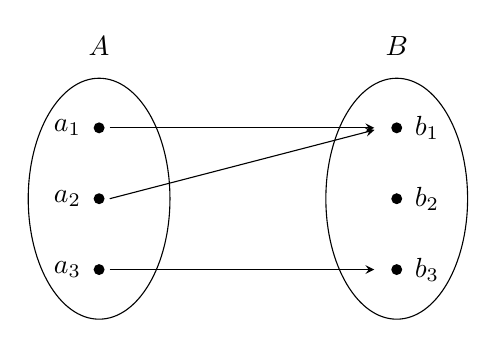
\begin{tikzpicture}[scale=0.9]
  \draw (0,0) ellipse (1 and 1.7);
  \draw (4.2,0) ellipse (1 and 1.7);
  \node at (0,2.15) {$A$};
  \node at (4.2,2.15) {$B$};
  \fill (0,1.0) circle (2.2pt) node[left=3pt] {$a_1$};
  \fill (0,0.0) circle (2.2pt) node[left=3pt] {$a_2$};
  \fill (0,-1.0) circle (2.2pt) node[left=3pt] {$a_3$};
  \fill (4.2,1.0) circle (2.2pt) node[right=3pt] {$b_1$};
  \fill (4.2,0.0) circle (2.2pt) node[right=3pt] {$b_2$};
  \fill (4.2,-1.0) circle (2.2pt) node[right=3pt] {$b_3$};
  \draw[->,>=stealth,shorten >=3pt] (0.15,1.0) -- (4.0,1.0);
  \draw[->,>=stealth,shorten >=3pt] (0.15,0.0) -- (4.0,1.0);
  \draw[->,>=stealth,shorten >=3pt] (0.15,-1.0) -- (4.0,-1.0);
\end{tikzpicture}
\end{center}

\noindent
এটি একটি বৈধ function: বাঁ পাশের প্রতিটি বিন্দু থেকে ঠিক একটি করে তীর
বেরিয়েছে। লক্ষ করো, $b_2$-তে কোনো তীর আসেনি, আর $b_1$-তে দুটো তীর এসেছে ---
এতে সংজ্ঞা ভাঙে না। শর্তটা কেবল বাঁ পাশ নিয়ে।

\begin{center}
\begin{tikzpicture}[scale=0.9]
  % failure 1: two arrows out
  \draw (0,0) ellipse (0.85 and 1.5);
  \draw (3.4,0) ellipse (0.85 and 1.5);
  \fill (0,0.7) circle (2.2pt) node[left=3pt] {$a_1$};
  \fill (0,-0.7) circle (2.2pt) node[left=3pt] {$a_2$};
  \fill (3.4,0.7) circle (2.2pt);
  \fill (3.4,-0.7) circle (2.2pt);
  \draw[->,>=stealth,shorten >=3pt] (0.12,0.7) -- (3.25,0.7);
  \draw[->,>=stealth,shorten >=3pt] (0.12,0.7) -- (3.25,-0.7);
  \node at (1.7,-2.1) {দোটানা};
  % failure 2: no arrow out
  \begin{scope}[xshift=6.6cm]
    \draw (0,0) ellipse (0.85 and 1.5);
    \draw (3.4,0) ellipse (0.85 and 1.5);
    \fill (0,0.7) circle (2.2pt) node[left=3pt] {$a_1$};
    \fill (0,-0.7) circle (2.2pt) node[left=3pt] {$a_2$};
    \fill (3.4,0.7) circle (2.2pt);
    \fill (3.4,-0.7) circle (2.2pt);
    \draw[->,>=stealth,shorten >=3pt] (0.12,0.7) -- (3.25,0.7);
    \node at (1.7,-2.1) {বাদ পড়া};
  \end{scope}
\end{tikzpicture}
\end{center}

\noindent
বাঁয়েরটিতে $a_1$ থেকে দুটো তীর বেরিয়েছে, ডানেরটিতে $a_2$ থেকে একটাও বেরোয়নি।
দুটোর কোনোটিই function নয়।


% ============================================================================
\section{ডোমেইন, কো-ডোমেইন, রেঞ্জ}
% ============================================================================

\begin{idea}[তিনটি সেট]
$f \colon A \to B$ একটি function হলে
\begin{itemize}
  \item $A$-কে বলে $f$-এর domain,
  \item $B$-কে বলে $f$-এর codomain,
  \item আর $\{\, f(a) : a \in A \,\}$ set-টিকে বলে $f$-এর range। অর্থাৎ, codomain-এর যেসব উপাদান domain-এর কোনো না কোনো উপাদানের সাথে সংশ্লিষ্ট তাদের সেটই range।
\end{itemize}
Range সবসময়ই codomain-এর একটি উপসেট, কিন্তু সেট দুটি সমান না-ও হতে পারে।

পার্থক্যটা ধরা জরুরি। Codomain তুমি বেছে নাও; ওটা তোমার ঘোষণা, ``output
এই set-এর ভেতরে পাবে''। Range তুমি বেছে নিতে পারো না; ওটা function আর domain
মিলে যা দাঁড়ায়, তা-ই। Codomain সিদ্ধান্ত, range ফলাফল।
\end{idea}

\begin{idea}[একটি function মানে তিনটি জিনিস]
একটি function সম্পূর্ণভাবে বলতে গেলে তিনটি জিনিস বলতে হয়: domain, codomain,
আর নিয়ম। তিনটির যেকোনো একটি বদলে গেলে function-টিও বদলে যায়, এমনকি সূত্রটা
হুবহু এক থাকলেও।

তাই ``$f(x) = x^2$ function-টি'' -একথাটা আসলে অসম্পূর্ণ। সূত্র এক হলেও $f \colon \mathbb{R} \to
\mathbb{R}$, আর $f \colon [0,\infty) \to [0,\infty)$ - এরা
আলাদা দুটি function বর্ণনা করবে, আর পরের অনুচ্ছেদে দেখব এদের আচরণও সম্পূর্ণ আলাদা।
\end{idea}

\begin{idea}[স্বাভাবিক ডোমেইন]
বাস্তবে অনেক সময় কেবল সূত্রটাই দেওয়া থাকে, domain আলাদা করে বলা থাকে না।
তখন প্রথা হলো: domain ধরা হয় সেই সব বাস্তব $x$-এর set, যাদের জন্য সূত্রটি
একটি বাস্তব মান দেয়। একে বলে সেই সূত্রের natural domain।

বাস্তবে দু-রকম জায়গায় সমস্যা বাধে : হরে শূন্য এলে, আর বর্গমূলের ভেতরে
ঋণাত্মক সংখ্যা এলে।
\end{idea}

\begin{example}
নিচের প্রতিটির natural domain বের করো।
\[
  \text{(ক)}\ \ f(x) = \frac{1}{(x-1)(x-4)}
  \qquad\qquad
  \text{(খ)}\ \ g(x) = \sqrt{x^2 - 3x - 10}
\]
\end{example}

\begin{solbox}
(ক) হর শূন্য হয় $x = 1$ আর $x = 4$-এ, অন্য কোথাও কোনো অসুবিধা নেই। তাই
natural domain হলো $\mathbb{R}$ থেকে ওই দুটো সংখ্যা বাদ:
\[
  (-\infty, 1) \cup (1, 4) \cup (4, \infty).
\]

(খ) বর্গমূলের ভেতরের রাশিটি অঋণাত্মক হতে হবে। মধ্যপদ বিশ্লেষণ করে
\[
  x^2 - 3x - 10 = (x - 5)(x + 2) \geq 0.
\]
আগের অনুচ্ছেদের যুক্তিতেই: দুজনেই অঋণাত্মক হলে $x \geq 5$, দুজনেই অধনাত্মক
হলে $x \leq -2$। সুতরাং natural domain
\[
  (-\infty, -2] \cup [5, \infty).
\]
\end{solbox}

\begin{example}
$f(x) = \dfrac{x+1}{x+3}$-এর natural domain ও range বের করো।
\end{example}

\begin{solbox}
হর শূন্য হয় কেবল $x = -3$-এ, তাই domain হলো
$(-\infty, -3) \cup (-3, \infty)$।

Range বের করার একটা সোজা কৌশল আছে : নিজেকে জিজ্ঞেস করো, কোন কোন $y$-এর জন্য
$f(x) = y$ সমীকরণটির একটা সমাধান আছে? $y$-কে ধ্রুবক ধরে $x$-এর জন্য সমাধান
করি:
\[
  y = \frac{x+1}{x+3}
  \ \Longrightarrow\ y(x + 3) = x + 1
  \ \Longrightarrow\ xy - x = 1 - 3y
  \ \Longrightarrow\ x(y - 1) = 1 - 3y .
\]
$y \neq 1$ হলে ভাগ করে পাই $x = \dfrac{1 - 3y}{y - 1}$, অর্থাৎ সমাধান আছে।
আর $y = 1$ হলে সমীকরণটি দাঁড়ায় $0 = -2$, যা কখনোই সত্য নয়। তাই $1$
কোনোভাবেই output হতে পারে না।

সুতরাং range $= (-\infty, 1) \cup (1, \infty)$।
\end{solbox}

\begin{remark}
একটা ফাঁদ, যেটায় প্রায় সবাই একবার না একবার পড়ে। ধরো
\[
  f(x) = \frac{x^2 - 9}{x - 3}.
\]
লব উৎপাদকে ভেঙে $x - 3$ কেটে দিলে থাকে $x + 3$। কিন্তু $f$ আর $x + 3$
\emph{একই function নয়}: $f$-এর domain-এ $x = 3$ নেই, অথচ $x + 3$ সূত্রটির
natural domain গোটা $\mathbb{R}$। ভাগ করার মুহূর্তেই তুমি ধরে নিয়েছিলে
$x \neq 3$, তাই সরলীকরণের সময়ে domain-টা চুপচাপ বদলে গেছে।

ঠিক লেখাটা হলো $f(x) = x + 3$, যেখানে $x \neq 3$। পদার্থবিজ্ঞানে এই ভুলটার
দাম চড়া; অনেক সময় ঠিক ওই বাদ পড়া বিন্দুটাতেই আসল ঘটনাটা ঘটে।
\end{remark}

% ============================================================================
\section{এক-এক ও সার্বিক}
% ============================================================================

আগের অনুচ্ছেদের সংজ্ঞা বাঁ পাশ নিয়ে দুটো শর্ত দিয়েছিল। এবার ডান পাশ নিয়ে
দুটো প্রশ্ন করি। প্রতিটি output কি সর্বোচ্চ একবার আসে? আর প্রতিটি output কি
অন্তত একবার আসে? দুটো প্রশ্ন সম্পূর্ণ আলাদা, আর দুটোরই আলাদা নাম আছে।

\begin{idea}[এক-এক ফাংশন]
$f \colon A \to B$-কে injective বা এক-এক (one to one) বলা হয়, যদি ভিন্ন input সবসময় ভিন্ন
output দেয়। সমানভাবে লেখা যায়: $A$-এর যেকোনো $x_1, x_2$-এর জন্য
\[
  f(x_1) = f(x_2) \ \Longrightarrow\ x_1 = x_2 .
\]
ছবির ভাষায়: $B$-এর কোনো বিন্দুতে একাধিক তীর এসে পড়ে না।
\end{idea}

\begin{idea}[সার্বিক ফাংশন]
$f \colon A \to B$-কে surjective বা সার্বিক (onto) বলা হয়, যদি $B$-এর প্রতিটি উপাদান
অন্তত একবার output হিসেবে আসে। অর্থাৎ প্রতিটি $b \in B$-এর জন্য এমন অন্তত
একটি $a \in A$ আছে যে $f(a) = b$।

সংক্ষেপে: $f$ surjective $\iff$ range $= $ codomain। ছবির ভাষায়: $B$-এর কোনো
বিন্দু তীরবিহীন থাকে না।
\end{idea}

\begin{idea}[বাইজেকশন]
যে function একই সঙ্গে injective ও surjective, তাকে বলে bijective, বা
এক-এক ও সার্বিক। এই ক্ষেত্রে $B$-এর প্রতিটি উপাদানে ঠিক একটি করে তীর এসে
পড়ে; একটিও কম নয়, একটিও বেশি নয়। $A$ ও $B$-এর উপাদানগুলো তখন নিখুঁতভাবে
জোড়ায় জোড়ায় সাজানো।
\end{idea}

\begin{center}
\begin{tikzpicture}[scale=0.82]
  % injective not surjective
  \draw (0,0) ellipse (0.8 and 1.5);
  \draw (2.9,0) ellipse (0.8 and 1.5);
  \fill (0,0.6) circle (2pt);
  \fill (0,-0.6) circle (2pt);
  \fill (2.9,1.0) circle (2pt);
  \fill (2.9,0.0) circle (2pt);
  \fill (2.9,-1.0) circle (2pt);
  \draw[->,>=stealth,shorten >=3pt] (0.12,0.6) -- (2.75,1.0);
  \draw[->,>=stealth,shorten >=3pt] (0.12,-0.6) -- (2.75,0.0);
  \node at (1.45,-2.15) {এক-এক, কিন্তু সার্বিক নয়};
  % surjective not injective
  \begin{scope}[xshift=5.6cm]
    \draw (0,0) ellipse (0.8 and 1.5);
    \draw (2.9,0) ellipse (0.8 and 1.5);
    \fill (0,1.0) circle (2pt);
    \fill (0,0.0) circle (2pt);
    \fill (0,-1.0) circle (2pt);
    \fill (2.9,0.6) circle (2pt);
    \fill (2.9,-0.6) circle (2pt);
    \draw[->,>=stealth,shorten >=3pt] (0.12,1.0) -- (2.75,0.6);
    \draw[->,>=stealth,shorten >=3pt] (0.12,0.0) -- (2.75,0.6);
    \draw[->,>=stealth,shorten >=3pt] (0.12,-1.0) -- (2.75,-0.6);
    \node at (1.45,-2.15) {সার্বিক, কিন্তু এক-এক নয়};
  \end{scope}
  % bijective
  \begin{scope}[xshift=11.2cm]
    \draw (0,0) ellipse (0.8 and 1.5);
    \draw (2.9,0) ellipse (0.8 and 1.5);
    \fill (0,0.8) circle (2pt);
    \fill (0,0.0) circle (2pt);
    \fill (0,-0.8) circle (2pt);
    \fill (2.9,0.8) circle (2pt);
    \fill (2.9,0.0) circle (2pt);
    \fill (2.9,-0.8) circle (2pt);
    \draw[->,>=stealth,shorten >=3pt] (0.12,0.8) -- (2.75,0.0);
    \draw[->,>=stealth,shorten >=3pt] (0.12,0.0) -- (2.75,-0.8);
    \draw[->,>=stealth,shorten >=3pt] (0.12,-0.8) -- (2.75,0.8);
    \node at (1.45,-2.15) {এক-এক এবং সার্বিক};
  \end{scope}
\end{tikzpicture}
\end{center}

\begin{example}
নিচের তিনটি ক্ষেত্রে নিয়ম একটাই : $x \mapsto x^2$। প্রতিটির জন্য বলো এটি
injective কি না, surjective কি না।
\[
  \text{(ক)}\ f \colon \mathbb{R} \to \mathbb{R}
  \qquad
  \text{(খ)}\ g \colon \mathbb{R} \to [0, \infty)
  \qquad
  \text{(গ)}\ h \colon [0, \infty) \to [0, \infty)
\]
\end{example}

\begin{solbox}
(ক) Injective নয়: $f(3) = 9 = f(-3)$, অথচ $3 \neq -3$। Surjective-ও নয়:
$-1 \in \mathbb{R}$ codomain-এ আছে, কিন্তু কোনো বাস্তব সংখ্যার বর্গ $-1$ হয়
না। অর্থাৎ range $= [0,\infty)$, যা codomain $\mathbb{R}$-এর চেয়ে ছোট।

(খ) Codomain ছোট করে ঠিক range-এর সমান করে দেওয়া হয়েছে, তাই এখন surjective:
যেকোনো $y \geq 0$-এর জন্য $x = \sqrt{y}$ নিলেই $g(x) = y$। কিন্তু domain
বদলায়নি, তাই এখনো injective নয় --- $g(3) = g(-3)$ সমস্যাটা রয়েই গেছে।

(গ) Domain-ও ছোট করে দেওয়া হয়েছে। এখন $x_1, x_2 \geq 0$ এবং
$x_1^2 = x_2^2$ হলে $x_1 = x_2$ হতেই হবে, কারণ দুজনেই অঋণাত্মক। তাই injective।
Surjective-ও, ঠিক (খ)-এর যুক্তিতে। সুতরাং $h$ একটি bijection।
\end{solbox}

\begin{remark}
উপরের উদাহরণটাই এই অনুচ্ছেদের মূল কথা। ``$x^2$ function-টি এক-এক কি না''
--- এই প্রশ্নটার কোনো উত্তর নেই, কারণ প্রশ্নটাই অসম্পূর্ণ। Domain আর codomain
না বললে injective বা surjective কথাগুলোর কোনো মানেই দাঁড়ায় না।

একটা সতর্কবার্তা, কারণ তুমি Stewart বা Anton-এর বই খুললেই এর মুখোমুখি হবে। ওই বইগুলো
codomain কথাটা আলাদা করে ব্যবহারই করে না ; ওরা নীরবে ধরে নেয় codomain মানেই
range। তাই তাঁদের বইয়ে লেখা থাকে ``$f$-এর inverse আছে যদি এবং কেবল যদি $f$
এক-এক হয়'' (পরের অনুচ্ছেদে inverse-এর অর্থ বুঝতে পারবে)। ওই প্রথায় কথাটা ঠিক, কারণ ওখানে surjective হওয়াটা ধরে নেওয়া হয়। কিন্তু এই সিরিজে আমরা codomain আলাদা করে বলছি, তাই আমাদের শর্তটা
দুটো এবং সেটাই পরের অনুচ্ছেদে প্রমাণ করা হবে। বই পড়ার সময় খেয়াল রেখো
লেখক কোন প্রথায় আছেন; দুটোই বৈধ, কিন্তু গুলিয়ে ফেললে ভুল হবেই।
\end{remark}

% ============================================================================
\section{বিপরীত ফাংশন}
% ============================================================================

\begin{idea}[কম্পোজিশন]
$f \colon A \to B$ আর $g \colon B \to C$ হলে, প্রথমে $f$ তারপর $g$ প্রয়োগ করে
$A$ থেকে $C$-তে একটি নতুন function পাওয়া যায়। একে বলে composition, লেখা হয়
$g \circ f$:
\[
  (g \circ f)(x) = g\big(f(x)\big), \qquad g \circ f \colon A \to C .
\]
লক্ষ করো, এটা কাজ করার জন্য $f$-এর codomain আর $g$-এর domain মিলতে হবে;
নইলে $g$ -কে যা খেতে দেওয়া হচ্ছে পাচ্ছে তা তার হজম হওয়ার কথা নয়।

আরও লক্ষ করো, $g \circ f$ হিসাব করতে হয় ডান থেকে বাঁয়ে: ভেতরেরটা আগে। আর
সাধারণভাবে $g \circ f \neq f \circ g$।
\end{idea}

\begin{idea}[অভেদ ফাংশন]
যেকোনো set $A$-এর জন্য $\mathrm{id}_A \colon A \to A$ function-টি সংজ্ঞায়িত হয়
$\mathrm{id}_A(x) = x$ দিয়ে। একে বলে $A$-এর identity function। এফাংশনশটি আসলে যা ইনপুট নেয়, তাই আউটপুট দেয়।
\end{idea}

\begin{idea}[বিপরীত ফাংশন (Inverse Function)]
$f \colon A \to B$-কে invertible বলা হয়, যদি এমন একটি function
$g \colon B \to A$ থাকে যে
\[
  g \circ f = \mathrm{id}_A \quad \text{এবং} \quad f \circ g = \mathrm{id}_B ,
\]
অর্থাৎ $g(f(a)) = a$ সব $a \in A$-এর জন্য, এবং $f(g(b)) = b$ সব $b \in B$-এর
জন্য। এমন $g$ থাকলে সেটি একটিই হয়, তাকে লেখা হয় $f^{-1}$। সহজভাবে,  $f$ ও $g$ যদি পরস্পরের বিপরীত ফাংশন হয়, তাহলে $f$-এ ইনপুট হিসেবে $a$ দিয়ে যে আউটপুট $f(a)$ পাওয়া যায় তাকেই যদি আবার $g$ ফাংশনে ইনপুট হিসেবে দেওয়া হয়, তাহলে আউটপুট হিসেবে আবার $a$-ই ফিরে আসে। একইভাবে $g$-তে কোনো ইনপুট দিয়ে প্রাপ্ত আউটপুটকে $f$-এর ইনপুট হিসেবে ব্যবহার করলে $f$ হতে প্রাপ্ত আউটপুট $g$-এর ইনপুটের সমান হয়। তাই $g=f^{-1}$ এবং $f=g^{-1}$।
\end{idea}

\begin{idea}[কখন বিপরীত থাকে]
$f \colon A \to B$ invertible (বিপরীতযোগ্য) হবে যদি এবং কেবল যদি $f$ bijective হয়।
\end{idea}

\noindent
\textbf{প্রমাণ।} দুই দিক আলাদা করে দেখি।

\emph{ধরি $f$ bijective।} যেকোনো $b \in B$ নাও। $f$ surjective, তাই এমন
অন্তত একটি $a \in A$ আছে যে $b=f(a)$। আবার $f$ injective, তাই এরকম $a$
একটির বেশি থাকতে পারে না। সুতরাং প্রতিটি $b$-এর জন্য ঠিক একটি $a$ আছে, আর
$g(b) = a$ লিখে দিলেই $g$ একটা বৈধ function হয়ে যায়। গড়ন থেকেই
$g(f(a)) = a$ এবং $f(g(b)) = b$।

লক্ষ করো, দুটো শর্তই ঠিক একবার করে লাগল: surjective না হলে $g$ কিছু জায়গায়
সংজ্ঞায়িতই হতো না (বাদ পড়া), আর injective না হলে $g$ কিছু জায়গায় দুটো মান
পেত (দোটানা)। এই দুটোই তো function-এর সংজ্ঞার সেই দুই শর্ত।

\emph{ধরি $f$ invertible, অর্থাৎ উপরের মতো $g$ আছে।} $f(x_1) = f(x_2)$ হলে
দুই পাশে $g$ প্রয়োগ করে $g(f(x_1)) = g(f(x_2))$, অর্থাৎ $x_1 = x_2$ ---
তাই $f$ injective। আবার যেকোনো $b \in B$-এর জন্য $f(g(b)) = b$, অর্থাৎ
$g(b)$ হলো সেই input যা $b$ দেয়। তাই $f$ surjective। $\blacksquare$

\begin{example}
দেখাও যে, $f \colon \mathbb{R} \to \mathbb{R}$, $f(x) = 3x - 7$ একটি bijection এবং $f^{-1}$ বের করো।
\end{example}

\begin{solbox}
\emph{Injective:} $3x_1 - 7 = 3x_2 - 7$ হলে দুই পাশে $7$ যোগ করে $3$ দিয়ে
ভাগ করলেই $x_1 = x_2$।

\emph{Surjective:} যেকোনো $y \in \mathbb{R}$ নাও। $x = \dfrac{y+7}{3}$ ধরলে
\[
  f(x) = 3 \cdot \frac{y+7}{3} - 7 = y .
\]
সুতরাং $f$ bijective, আর
\[
  f^{-1}(y) = \frac{y + 7}{3}.
\]

মিলিয়ে দেখি: $f^{-1}(f(x)) = \dfrac{(3x - 7) + 7}{3} = x$ এবং
$f(f^{-1}(y)) = 3 \cdot \dfrac{y+7}{3} - 7 = y$। দুটোই ঠিক।

খেয়াল করো, কাজটা আসলে অধ্যায় ২-এর সেই পুরোনো কাজ : $y = 3x - 7$
সমীকরণটি $x$-এর জন্য সমাধান করা। নতুন যা, তা হলো উত্তরটাকে একটা নতুন
function হিসেবে দেখা।
\end{solbox}

\begin{example}
$h \colon [0, \infty) \to [0, \infty)$, $h(x) = x^2$-এর inverse বের করো।
\end{example}

\begin{solbox}
আগের অনুচ্ছেদে দেখেছি এই $h$ bijective, তাই inverse আছে। $y = x^2$ এবং
$x \geq 0$ হলে $x = \sqrt{y}$। সুতরাং
\[
  h^{-1} \colon [0, \infty) \to [0, \infty), \qquad h^{-1}(y) = \sqrt{y}.
\]
Domain সংকুচিত না করলে এটা করা যেত না --- $f \colon \mathbb{R} \to \mathbb{R}$,
$f(x) = x^2$-এর কোনো inverse নেই, কারণ $f^{-1}(9)$-এর মান $3$ না $-3$ তা ঠিক
করার কোনো উপায় নেই।
\end{solbox}

\begin{remark}
$f^{-1}$ লেখাটায় $-1$ কোনো ঘাত নয়। $f^{-1}(x)$ আর $\dfrac{1}{f(x)}$ সম্পূর্ণ
আলাদা দুটো জিনিস, আর এদের গুলিয়ে ফেলা সম্ভবত এই অধ্যায়ের সবচেয়ে
প্রচলিত ভুল।

Inverse-এর ধারণাটা সামনে বারবার ফিরে আসবে। অধ্যায় ৮-এ logarithm আসবে সূচকীয় function-এর inverse হিসেবে; আর তখন domain আর codomain কী কী
বেছে নিলে ওই inverse-টা আদৌ থাকে, সেই প্রশ্নটাই মুখ্য হয়ে উঠবে।
\end{remark}

% ============================================================================
\section{খণ্ডিত ফাংশন}
% ============================================================================

\begin{idea}[খণ্ডিত ফাংশন]
কোনো function-এর নিয়ম domain-এর সব উপাদানের জন্য একই হতে হবে; এমন কোনো কথা নেই।
Domain-কে কয়েক টুকরো করে প্রতি টুকরোয় আলাদা সূত্র দিলে যে function পাওয়া যায়,
তাকে বলে piecewise বা খণ্ডিত function। যেসব বিন্দুতে সূত্র বদলায়, তাদের বলে
breakpoint।

শর্ত একটাই, আর সেটা function-এর সেই মূল সংজ্ঞাই: টুকরোগুলো মিলে গোটা domain
ঢেকে দিতে হবে (domain-এর এক্বটি উপাদানও বাদ পড়া চলবে না), আর কোনো $x$ যেন দুটো টুকরোয় একসঙ্গে পড়ে
দুটো ভিন্ন মান না পায় (দোটানা চলবে না)। ভাগ করার সময় $\leq$ আর $<$ কোথায়
বসছে, সেটা তাই খুঁটিয়ে দেখতে হয়।
\end{idea}

\begin{idea}[পরম মান]
সবচেয়ে চেনা খণ্ডিত function হলো পরম মান:
\[
  |x| =
  \begin{cases}
    x, & x \geq 0, \\[2pt]
    -x, & x < 0 .
  \end{cases}
\]
দুটো টুকরো মিলে গোটা $\mathbb{R}$ কভার করেছে, আর কোথাও একে অপরের উপর পড়েনি।
তাই সংজ্ঞাটি বৈধ।
\end{idea}

\begin{example}
দেখাও যে সব বাস্তব $x$-এর জন্য $\sqrt{x^2} = |x|$, এবং ব্যাখ্যা করো কেন
$\sqrt{x^2} = x$ লেখাটা ভুল।
\end{example}

\begin{solbox}
মনে রেখো, $\sqrt{\ }$ চিহ্নটি সবসময় কোনো সংখ্যার অঋণাত্মক বর্গমূলটিকে বোঝায়। তাই
$\sqrt{x^2}$ কখনোই ঋণাত্মক হতে পারে না।

$x \geq 0$ হলে $x$ নিজেই অঋণাত্মক এবং $x^2$-এর বর্গমূল, তাই
$\sqrt{x^2} = x = |x|$।

$x < 0$ হলে $x$ ঋণাত্মক, তাই সে $\sqrt{x^2}$ হতে পারে না। কিন্তু $-x$
ধনাত্মক এবং $(-x)^2 = x^2$, তাই $\sqrt{x^2} = -x = |x|$।

দুই ক্ষেত্রেই $\sqrt{x^2} = |x|$।

$\sqrt{x^2} = x$ লেখাটা তাই কেবল $x \geq 0$-এর জন্য সত্য। $x = -5$ বসিয়ে
দেখো: বাঁ পাশ $\sqrt{25} = 5$, ডান পাশ $-5$। অধ্যায় ১-এর ভাষায়, এই
একটামাত্র counterexample-ই দাবিটাকে মেরে ফেলার জন্য যথেষ্ট।
\end{solbox}

\begin{example}
$f \colon \mathbb{R} \to \mathbb{R}$ সংজ্ঞায়িত
\[
  f(x) =
  \begin{cases}
    2x, & x \leq 1, \\[2pt]
    x^2 + 1, & x > 1 .
  \end{cases}
\]
$f(-3)$, $f(1)$, $f(3)$ বের করো, এবং $f$ injective কি না বলো।
\end{example}

\begin{solbox}
$-3 \leq 1$, তাই প্রথম সূত্র: $f(-3) = -6$।

$1 \leq 1$, তাই এখানেও প্রথম সূত্র: $f(1) = 2$। (এই কারণেই breakpoint-এ
কোন সূত্রটি খাটবে তা আগেই ঠিক করে বলে দিতে হয়।)

$3 > 1$, তাই দ্বিতীয় সূত্র: $f(3) = 10$।

Injective কি না দেখতে দুটো টুকরো আলাদা করে, তারপর একসঙ্গে দেখতে হয়।
$(-\infty, 1]$-এ $f(x) = 2x$, আর $2x_1 = 2x_2$ হলে $x_1 = x_2$ --- এই টুকরোয়
injective, আর এখানকার মানগুলো $(-\infty, 2]$ জুড়ে ছড়ানো। $(1, \infty)$-এ
$f(x) = x^2 + 1$, আর $x_1, x_2 > 1$ হলে $x_1^2 = x_2^2$ থেকে $x_1 = x_2$ ---
এখানেও injective, আর এখানকার মানগুলো $(2, \infty)$-এ পড়ে।

দুটো output set-এর মধ্যে কোনো মিল বা সাধারণ অংশ নেই, তাই দুই টুকরো থেকে একই output আসার
সুযোগও নেই। সুতরাং $f$ injective।
\end{solbox}

\begin{remark}
খণ্ডিত function-কে ``জোড়াতালি'' ভাবার কোনো কারণ নেই; পদার্থবিজ্ঞানে এরা
সর্বত্র। কোনো আধানযুক্ত গোলকের ভেতরে আর বাইরে বৈদ্যুতিক ক্ষেত্রের সূত্র
আলাদা, কোনো স্প্রিং-এর সংকোচন আর প্রসারণে আচরণ আলাদা।

Breakpoint-এ কী ঘটে; মান কি লাফ দেয়, না মসৃণভাবে জোড়া লাগে : এই
প্রশ্নটার নাম continuity, আর সেটাই অধ্যায় ১৫-এর মূল বিষয়। $|x|$
function-টি তখন আবার ফিরবে, একটা বিখ্যাত উদাহরণ হয়ে: $x = 0$-তে সে
continuous, অথচ differentiable নয়।
\end{remark}


% ============================================================================
\section{সমস্যা}
% ============================================================================

\prob{1} নিচের set-গুলো ব্যবধির ভাষায় লেখো।
\begin{enumerate}
  \item $\{\, x \in \mathbb{R} : -2 \leq x < 5 \,\}$
  \item $\{\, x \in \mathbb{R} : x > 3 \,\}$
  \item $\{\, x \in \mathbb{R} : x^2 \leq 9 \,\}$
\end{enumerate}

\begin{sol}
\begin{enumerate}
  \item $[-2, 5)$
  \item $(3, \infty)$
  \item $x^2 \leq 9$ মানে $|x| \leq 3$, অর্থাৎ $-3 \leq x \leq 3$; সুতরাং
        $[-3, 3]$।
\end{enumerate}
\end{sol}

\prob{2} নিচের প্রতিটির natural domain বের করো।
\begin{enumerate}
  \item $f(x) = \dfrac{x + 4}{x^2 - 9}$
  \item $g(x) = \sqrt{2x - 7}$
\end{enumerate}

\begin{sol}
\begin{enumerate}
  \item $x^2 - 9 = (x-3)(x+3)$ শূন্য হয় $x = \pm 3$-এ, তাই domain
        $(-\infty, -3) \cup (-3, 3) \cup (3, \infty)$।
  \item $2x - 7 \geq 0$, অর্থাৎ $x \geq \tfrac{7}{2}$; domain
        $\left[\tfrac{7}{2}, \infty\right)$।
\end{enumerate}
\end{sol}

\prob{2} $h(x) = \sqrt{x^2 - 7x + 10} + \dfrac{1}{x - 6}$-এর natural domain
বের করো।

\begin{sol}
দুটো শর্ত একসঙ্গে মানতে হবে।

বর্গমূলের জন্য $(x-2)(x-5) \geq 0$, যা প্রথম অনুচ্ছেদের উদাহরণে করা হয়েছে:
$x \leq 2$ অথবা $x \geq 5$।

ভগ্নাংশের জন্য $x \neq 6$।

দুটো মিলিয়ে domain
\[
  (-\infty, 2] \cup [5, 6) \cup (6, \infty).
\]
\end{sol}

\prob{2} নিচের কোন নিয়মগুলো $\mathbb{R}$ থেকে $\mathbb{R}$-এ একটি function
সংজ্ঞায়িত করে? যেগুলো করে না, কোন শর্তটি ভাঙছে তা বলো।
\begin{enumerate}
  \item $f(x) = x^3$
  \item ``$y$ এমন যে $y^3 = x$''
  \item $f(x) = \dfrac{1}{x}$
  \item $f(x) = |x|$
\end{enumerate}

\begin{sol}
\begin{enumerate}
  \item হ্যাঁ। প্রতিটি বাস্তব $x$-এর জন্য $x^3$ একটিই বাস্তব সংখ্যা।
  \item হ্যাঁ। প্রতিটি বাস্তব $x$-এর ঠিক একটি বাস্তব ঘনমূল আছে --- বর্গমূলের
        মতো এখানে দোটানা নেই, কারণ ঋণাত্মক সংখ্যারও ঘনমূল আছে এবং সেটি
        একটিই।
  \item না। $x = 0$-তে কোনো মান নেই, অর্থাৎ domain $\mathbb{R}$-এর একটি
        উপাদান বাদ পড়ে গেছে। তবে $\mathbb{R} \setminus \{0\}$ থেকে
        $\mathbb{R}$-এ এটি একটি বৈধ function।
  \item হ্যাঁ। খণ্ডিতভাবে সংজ্ঞায়িত হলেও দুই টুকরো মিলে গোটা $\mathbb{R}$
        ঢেকেছে এবং কোথাও দোটানা নেই।
\end{enumerate}
\end{sol}

\prob{2} $f \colon \mathbb{R} \to \mathbb{R}$, $f(x) = 5 - 2x$। দেখাও এটি
bijective, এবং $f^{-1}$ বের করো।

\begin{sol}
\emph{Injective:} $5 - 2x_1 = 5 - 2x_2$ হলে $-2x_1 = -2x_2$, অর্থাৎ
$x_1 = x_2$।

\emph{Surjective:} যেকোনো $y \in \mathbb{R}$-এর জন্য $x = \dfrac{5 - y}{2}$
নিলে
\[
  f(x) = 5 - 2 \cdot \frac{5-y}{2} = 5 - (5 - y) = y .
\]

সুতরাং $f$ bijective এবং $f^{-1}(y) = \dfrac{5 - y}{2}$।
\end{sol}

\prob{3} $f(x) = x^2 - 4x$ ধরো।
\begin{enumerate}
  \item $f \colon \mathbb{R} \to \mathbb{R}$ injective কি না বলো।
  \item এখন domain সংকুচিত করে $[2, \infty)$ করা হলো। দেখাও যে এই
        function-টি injective, এবং এর range বের করো।
\end{enumerate}

\begin{sol}
\begin{enumerate}
  \item না। $f(0) = 0$ এবং $f(4) = 16 - 16 = 0$, অথচ $0 \neq 4$।
  \item বর্গ পূর্ণ করে লিখি:
        \[
          f(x) = x^2 - 4x + 4 - 4 = (x-2)^2 - 4 .
        \]
        $x_1, x_2 \geq 2$ এবং $f(x_1) = f(x_2)$ হলে $(x_1 - 2)^2 =
        (x_2 - 2)^2$। এখানে $x_1 - 2$ ও $x_2 - 2$ দুটোই অঋণাত্মক, তাই
        $x_1 - 2 = x_2 - 2$, অর্থাৎ $x_1 = x_2$। সুতরাং injective।

        Range বের করতে $u = x - 2$ বসাই। $x$ যখন $[2, \infty)$ জুড়ে চলে,
        $u$ তখন $[0, \infty)$ জুড়ে চলে, ফলে $u^2$ চলে $[0, \infty)$ জুড়ে,
        আর $u^2 - 4$ চলে $[-4, \infty)$ জুড়ে। সুতরাং range $= [-4, \infty)$।
\end{enumerate}
\end{sol}

\prob{3} $g(x) = x^2 + 1$ ধরো।
\begin{enumerate}
  \item দেখাও যে $g \colon \mathbb{R} \to \mathbb{R}$ surjective নয়।
  \item codomain কী নিলে এটি surjective হয়?
  \item সেই codomain রেখে domain কী নিলে এটি bijective হয়?
\end{enumerate}

\begin{sol}
\begin{enumerate}
  \item সব বাস্তব $x$-এর জন্য $x^2 \geq 0$, তাই $g(x) \geq 1$। সুতরাং
        $0 \in \mathbb{R}$ কখনোই output হয় না, অথচ সে codomain-এ আছে।
  \item Range-টাই বের করি। $y \geq 1$ হলে $x = \sqrt{y - 1}$ নিলে
        $g(x) = (y-1) + 1 = y$, তাই এরা সবাই আসে; আর $y < 1$ কেউ আসে না।
        সুতরাং range $= [1, \infty)$, এবং $g \colon \mathbb{R} \to
        [1, \infty)$ surjective। তবু injective নয়, কারণ $g(2) = g(-2) = 5$।
  \item Domain $[0, \infty)$ নিলে: $x_1, x_2 \geq 0$ এবং $x_1^2 + 1 =
        x_2^2 + 1$ হলে $x_1^2 = x_2^2$, আর দুজনেই অঋণাত্মক বলে $x_1 = x_2$।
        সুতরাং $g \colon [0, \infty) \to [1, \infty)$ bijective।
        ($(-\infty, 0]$ নিলেও চলত।)
\end{enumerate}
\end{sol}

\prob{2} $f(x) = 2x + 1$ এবং $g(x) = x^2 - 3$, দুটোই $\mathbb{R} \to
\mathbb{R}$। $f \circ g$ ও $g \circ f$ বের করো, এবং একটি সংখ্যা দেখিয়ে
প্রমাণ করো যে এরা একই function নয়।

\begin{sol}
\[
  (f \circ g)(x) = f(x^2 - 3) = 2(x^2 - 3) + 1 = 2x^2 - 5 ,
\]
\[
  (g \circ f)(x) = g(2x + 1) = (2x+1)^2 - 3 = 4x^2 + 4x - 2 .
\]
$x = 0$ বসালে প্রথমটি দেয় $-5$, দ্বিতীয়টি দেয় $-2$। একটিমাত্র input-এ
ভিন্ন মান --- তাই এরা ভিন্ন function।
\end{sol}

\prob{3} $f \colon A \to B$ এবং $g \colon B \to C$ দুটি function।
\begin{enumerate}
  \item প্রমাণ করো: $f$ ও $g$ দুটোই injective হলে $g \circ f$ injective।
  \item প্রমাণ করো: $f$ ও $g$ দুটোই surjective হলে $g \circ f$ surjective।
\end{enumerate}

\begin{sol}
\begin{enumerate}
  \item ধরি $(g \circ f)(x_1) = (g \circ f)(x_2)$, অর্থাৎ
        $g(f(x_1)) = g(f(x_2))$। $g$ injective, তাই $f(x_1) = f(x_2)$।
        আবার $f$ injective, তাই $x_1 = x_2$।
  \item যেকোনো $c \in C$ নাও। $g$ surjective, তাই এমন $b \in B$ আছে যে
        $g(b) = c$। $f$ surjective, তাই এমন $a \in A$ আছে যে $f(a) = b$।
        তাহলে $(g \circ f)(a) = g(f(a)) = g(b) = c$।
\end{enumerate}

দুটো মিলিয়ে: দুটো bijection-এর composition আবার একটি bijection।
\end{sol}

\prob{3} $f \colon \mathbb{R} \setminus \{2\} \to \mathbb{R} \setminus \{1\}$,
$f(x) = \dfrac{x + 2}{x - 2}$। দেখাও এটি bijective এবং $f^{-1}$ বের করো।

\begin{sol}
প্রথমে দেখি codomain থেকে $1$ বাদ দেওয়া যুক্তিসঙ্গত: $f(x) = 1$ হলে
$x + 2 = x - 2$, অর্থাৎ $2 = -2$, যা অসম্ভব। তাই $1$ কখনোই output নয়।

এখন $y = \dfrac{x+2}{x-2}$ ধরে $x$ বের করি:
\[
  y(x - 2) = x + 2
  \ \Longrightarrow\ xy - x = 2y + 2
  \ \Longrightarrow\ x(y - 1) = 2y + 2 .
\]
$y \neq 1$, তাই ভাগ করা যায়:
\[
  x = \frac{2y + 2}{y - 1}.
\]
এই $x$ কখনো $2$ হয় না, কারণ $\dfrac{2y+2}{y-1} = 2$ হলে $2y + 2 = 2y - 4$,
অসম্ভব। সুতরাং $g(y) = \dfrac{2y+2}{y-1}$ সত্যিই $\mathbb{R} \setminus \{1\}$
থেকে $\mathbb{R} \setminus \{2\}$-এ একটি function।

যাচাই:
\[
  g(f(x)) = \frac{2 \cdot \frac{x+2}{x-2} + 2}{\frac{x+2}{x-2} - 1}
          = \frac{\frac{2(x+2) + 2(x-2)}{x-2}}{\frac{(x+2) - (x-2)}{x-2}}
          = \frac{4x}{4} = x .
\]
একইভাবে $f(g(y)) = y$। দুই দিকেই inverse পাওয়া গেল, তাই আগের অনুচ্ছেদের
উপপাদ্য অনুযায়ী $f$ bijective, এবং
\[
  f^{-1}(y) = \frac{2y + 2}{y - 1}.
\]
\end{sol}

\prob{2} $f \colon \mathbb{R} \to \mathbb{R}$ সংজ্ঞায়িত
\[
  f(x) =
  \begin{cases}
    x + 3, & x < -1, \\[2pt]
    x^2, & -1 \leq x \leq 2, \\[2pt]
    8 - 2x, & x > 2 .
  \end{cases}
\]
$f(-4)$, $f(-1)$, $f(0)$, $f(2)$, $f(5)$ বের করো। $f$ কি injective?

\begin{sol}
$-4 < -1$, তাই $f(-4) = -4 + 3 = -1$।

$-1$ দ্বিতীয় টুকরোয় পড়ে (কারণ শর্তটি $-1 \leq x$), তাই $f(-1) = (-1)^2 = 1$।

$f(0) = 0^2 = 0$ এবং $f(2) = 2^2 = 4$।

$5 > 2$, তাই $f(5) = 8 - 10 = -2$।

Injective নয়। $-1$ ও $1$ দুটোই $[-1, 2]$-এ পড়ে, আর
\[
  f(-1) = 1 = f(1),
\]
অথচ $-1 \neq 1$।
\end{sol}

\prob{3} $f \colon A \to B$ একটি function, এবং ধরি এমন একটি function
$g \colon B \to A$ আছে যে সব $a \in A$-এর জন্য $g(f(a)) = a$।
\begin{enumerate}
  \item প্রমাণ করো $f$ injective।
  \item একটি উদাহরণ দাও যেখানে এমন $g$ আছে অথচ $f$ surjective নয়।
\end{enumerate}

\begin{sol}
\begin{enumerate}
  \item ধরি $f(x_1) = f(x_2)$। দুই পাশে $g$ প্রয়োগ করে
        $g(f(x_1)) = g(f(x_2))$। শর্ত অনুযায়ী বাঁ পাশ $x_1$ আর ডান পাশ
        $x_2$, তাই $x_1 = x_2$।
  \item $A = [0, \infty)$, $B = \mathbb{R}$, $f(x) = x$ এবং $g(y) = |y|$
        নাও। সব $a \geq 0$-এর জন্য $g(f(a)) = |a| = a$, তাই শর্তটি মানা
        হয়েছে। কিন্তু $f$ surjective নয় --- codomain-এ $-1$ আছে, অথচ
        $f$-এর range কেবল $[0, \infty)$।
\end{enumerate}

এই সমস্যাটাই দেখাচ্ছে কেন inverse-এর সংজ্ঞায় \emph{দুটো} শর্ত লাগে। কেবল
$g \circ f = \mathrm{id}_A$ পেলে $g$-কে ``বাঁ দিকের inverse'' বলা যায়, কিন্তু
তাতে $f$-কে bijection বানানো যায় না। $f \circ g = \mathrm{id}_B$ শর্তটিই
surjectivity-র দায়িত্ব নেয়।
\end{sol}

\end{document}